% Drawing 146/02-3 -- folder 146, batch 02, archive page 32 (PDF page 33).
% Transcription: Une chaîne de points sur une courbe fermée, chacun muni de petites boucles fléchées (les lacets $\lambda$), reliés par des flèches à double sens. Au premier plan, en trait gras : $\widetilde{Q}_a \xrightarrow{\tilde b_r} \widetilde{R}_r$, puis un arc $\tilde a_r$ de $\widetilde{R}_r$ vers $\widetilde{R}_{r_1}$, sous lequel un arc $\tilde a_{r_1}$ ; au-dessus, un autre point avec l'arc $\tilde a_{r_1^\vee}$. La région entre $\widetilde{R}_r$, $\widetilde{Q}_a$ et un sommet commun est hachurée ; des traits fins portent $r$, $r_1$, $r_2$. Plus bas à droite, un petit triangle isolé.
% Kind: surface figure (chain of looped points, paths). Method 2 (schematic redraw from the facsimile). Status: partial.
% Notes: Closed chain of five looped points: each loop is two arrowed arcs round its point (since 2026-11-14), and the double arrows run along the straight segments between the points (top <-> top right, top <-> upper left, upper left <-> lower left as a curve on the left, top right <-> lower right as a curve on the right). From the lower left point the chain goes through the dot to R~r1 (arrows), from Q~a to the lower right point (arrow). The bold b~r runs from Q~a to R~r, the bold a~r is the upper half of an ellipse from R~r to R~r1 (arrow at R~r1), the thin a~r1 its lower half, so the two arcs share their end points. The hatched region is bounded by the line from the apex to the right, the arc a~r and the vertical from the apex; the faint lines from the apex to the lower left point and to the dot are drawn in pencil, with r, r1, r2 by them. Left out: the long horizontal rule across the top (a stroke of the page, not of the figure), the label above the top loop written on that rule (« a~r » with a mark? not certain), the arrowheads of the small loops, the small isolated triangle lower right (outside the bbox). The label a~_{r1^vee} is placed under the top loop, where « a r1 » with a check mark stands. Redrawn 2026-11-09 (issue 128): to check again. 2026-11-13, Claude Opus 5.5, overlay check (issue 147): rasterised from its own coordinates over the 400 dpi colour scan (250 ppi native) on a unit grid; the five looped points, the double arrows between them, the bold b~r and a~r, the thin a~r1, the hatched region and the faint lines from the apex lie on their ink to within 1 to 2 units, so the redraw is unchanged. Not compiled (no TeX in the session).  2026-11-14, Claude Opus 5.5, issue 147 second pass: the five small loops redrawn stroke by stroke from the 400 dpi scan on gridded crops at 26 pixels per unit: on the page none is a closed circle; each is an upper and a lower arc round its point, each arc with its own head (and a small tick on the chord inside the top loop), drawn where they stand; the five whole circles of the earlier redraw are gone. Overlay with the local TikZ interpreter (not compiled: no TeX in the session): the arcs and heads lie on their ink to within about one unit. Still differs: the hatching of the region between a~r and b~r is about fourteen separate pencil strokes at roughly 50 degrees, of uneven length, and is still drawn as a 45-degree pattern (not redrawn stroke by stroke in this pass); the label above the top loop, written on the long rule, is not settled.
% Coordinates: 1 unit = 1 mm = 1/100 of the crop width (bbox in page fractions: [0.13, 0.285, 0.5, 0.45]).
% Redrawn by Claude (claude-opus-5-5), issue #73, 2026-11-09; not checked by a human; not compiled (no TeX in the session).
% Checked by Claude (claude-opus-5-5) 2026-11-13 (issue #147): overlaid on the 400 dpi colour facsimile; not compiled (no TeX in the session). Not checked by a human. Status: partial.
% Rights: reproduces part of the work -- behind RENDER_TRANSCRIPTS, never published by itself.
\documentclass[tikz,border=3pt]{standalone}
\usepackage{amsmath,amssymb}
\usetikzlibrary{patterns,arrows.meta}
\tikzset{pencil/.style={black!45}, struck/.style={black!35}, mark/.style={circle,draw,inner sep=1.3pt}, pt/.style={circle,fill,inner sep=0.9pt}, opt/.style={circle,draw,fill=white,inner sep=1.1pt}}
\begin{document}
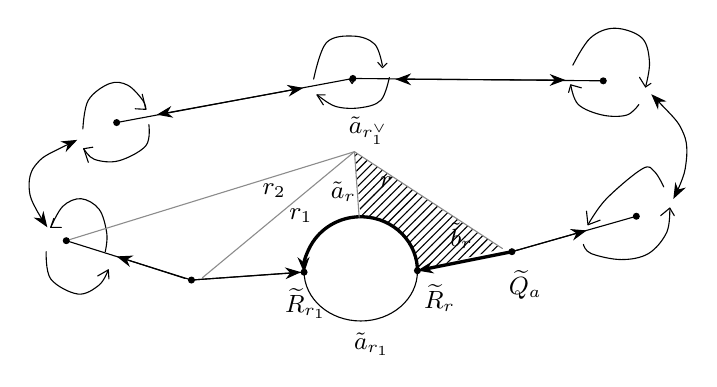
\begin{tikzpicture}[x=1mm,y=1mm,line cap=round,line join=round,font=\scriptsize]
% the five small loops: each two arcs with their heads, as on the page
\draw plot[smooth, tension=0.6] coordinates {(44.62,-19.08) (46.23,-14.46) (49.69,-13.62) (52.38,-14.65) (53.35,-17.35)};
\draw plot[smooth, tension=0.6] coordinates {(54.23,-18.88) (53.15,-21.77) (50.46,-22.73) (47.38,-22.54) (45.08,-21.08)};
\draw (52.77,-16.96) -- (53.35,-17.62) -- (53.92,-17.08);
\draw (46.08,-21.08) -- (45.04,-21.08) -- (45.85,-22.35);
\draw (49.12,-19.08) -- (49.5,-19.65) -- (49.88,-19.08);
\draw plot[smooth, tension=0.6] coordinates {(77.54,-17.31) (79.77,-13.85) (82.85,-12.62) (86.31,-13.85) (87.27,-16.92) (86.77,-20.08)};
\draw plot[smooth, tension=0.6] coordinates {(85.92,-22.31) (84.38,-23.65) (81.31,-23.65) (78.23,-22.31) (77.27,-19.81)};
\draw (86,-18.85) -- (86.77,-20.08) -- (87.46,-19.62);
\draw (78.62,-20.19) -- (77.27,-19.81) -- (77,-20.77);
\draw plot[smooth, tension=0.6] coordinates {(15.31,-25.42) (16,-21.77) (18.69,-19.65) (21,-19.85) (22.92,-21.77) (23.31,-22.92)};
\draw plot[smooth, tension=0.6] coordinates {(23.69,-24.85) (23.31,-27.54) (19.85,-29.46) (16.77,-29.27) (15.42,-27.92)};
\draw (22.85,-21) -- (23.31,-22.92) -- (21.96,-22.85);
\draw (16.58,-27.73) -- (15.42,-27.92) -- (16,-29.65);
\draw plot[smooth, tension=0.6] coordinates {(18.15,-41) (18.35,-38.69) (17.38,-35.62) (15.08,-34.27) (12.77,-35.23) (11.23,-37.92)};
\draw plot[smooth, tension=0.6] coordinates {(10.65,-41) (11.23,-44.46) (14.69,-46.38) (17.38,-45.23) (18.54,-43.31)};
\draw (12.58,-37.92) -- (11.23,-37.92) -- (11.62,-36.77);
\draw (17.19,-44.08) -- (18.54,-43.31) -- (18.62,-44.46);
\draw plot[smooth, tension=0.6] coordinates {(89.08,-32.77) (87.92,-30.85) (86.38,-30.46) (81.77,-34.31) (79.46,-37.58)};
\draw plot[smooth, tension=0.6] coordinates {(78.88,-40.08) (79.85,-41.23) (83.69,-42) (87.15,-41.23) (89.46,-38.54) (89.85,-35.46)};
\draw (79.27,-35.85) -- (79.46,-37.58) -- (81,-37);
\draw (88.69,-36.42) -- (89.85,-35.46) -- (90.42,-36.42);
\draw (49.6,-19) -- (81.4,-19.3);
\draw (49.6,-19) -- (19.6,-24.6);
\draw (13.2,-39.6) -- (29.1,-44.6) -- (43.4,-43.6);
\draw (69.8,-41) -- (85.6,-36.5);
\draw[{Stealth[length=2mm]}-{Stealth[length=2mm]}] (55,-19.1) -- (76.6,-19.2);
\draw[{Stealth[length=2mm]}-{Stealth[length=2mm]}] (43.3,-20.2) -- (24.7,-23.6);
\draw[{Stealth[length=2mm]}-{Stealth[length=2mm]}] plot[smooth, tension=0.55] coordinates {(14.6,-26.8) (9.3,-30) (8.6,-33.8) (10.8,-37.9)};
\draw[{Stealth[length=2mm]}-{Stealth[length=2mm]}] plot[smooth, tension=0.55] coordinates {(87.5,-21) (91.6,-26) (91.8,-30.5) (90.3,-34.3)};
\draw[-{Stealth[length=2mm]}] (28.3,-44.4) -- (19.6,-41.6);
\draw[-{Stealth[length=2mm]}] (29.1,-44.6) -- (43,-43.6);
\draw[-{Stealth[length=2mm]}] (69.8,-41) -- (79.3,-38.3);
\draw[very thick,-{Stealth[length=2mm]}] (69.8,-41) -- (57.8,-43.4);
\draw[very thick,-{Stealth[length=2mm]}] (57.8,-43.7) arc[start angle=-2, end angle=182, x radius=7.2, y radius=6.9];
\draw (43.4,-43.5) arc[start angle=180, end angle=360, x radius=7.2, y radius=6.3];
\fill[pattern=north east lines] (49.8,-28.3) -- (68.6,-40.6) -- (57.8,-43.4) -- (57,-40) -- (54,-37.2) -- (50.6,-36.6) -- cycle;
\draw[pencil] (49.8,-28.3) -- (68.6,-40.6);
\draw[pencil] (49.8,-28.3) -- (50.4,-36.6);
\draw[pencil] (49.8,-28.3) -- (13.2,-39.6);
\draw[pencil] (49.8,-28.3) -- (30.5,-44.3);
\node[pt] at (49.6,-19) {};
\node[pt] at (81.4,-19.3) {};
\node[pt] at (19.6,-24.6) {};
\node[pt] at (13.2,-39.6) {};
\node[pt] at (85.6,-36.5) {};
\node[pt] at (43.4,-43.6) {};
\node[pt] at (57.8,-43.4) {};
\node[pt] at (69.8,-41) {};
\node[pt] at (29.1,-44.6) {};
\node[inner sep=1pt] at (71.5,-45.2) {\small $\widetilde{Q}_a$};
\node[inner sep=1pt] at (60.6,-46.9) {\small $\widetilde{R}_r$};
\node[inner sep=1pt] at (43.6,-47.6) {\small $\widetilde{R}_{r_1}$};
\node[inner sep=1pt] at (48.4,-33.4) {\small $\tilde a_r$};
\node[inner sep=1pt] at (63.4,-39) {\small $\tilde b_r$};
\node[inner sep=1pt] at (52,-52.8) {\small $\tilde a_{r_1}$};
\node[inner sep=1pt] at (51.6,-25.6) {\small $\tilde a_{r_1^\vee}$};
\node[inner sep=1pt] at (53.8,-32.2) {\small $r$};
\node[inner sep=1pt] at (43,-36.4) {\small $r_1$};
\node[inner sep=1pt] at (39.6,-33.2) {\small $r_2$};
\end{tikzpicture}
\end{document}
